\documentclass[10 pt,usenames,dvipsnames, oneside]{article}
\usepackage{../../../modelo-ensino-medio}



\begin{document}

\begin{center}
  \begin{minipage}[l]{3cm}

\includegraphics[width=2cm]{logo}    
\end{minipage}\hfill
\begin{minipage}[r]{.8\textwidth}
 {\Large \scshape Atividade: Um cafézinho}  
\end{minipage}
\end{center}
\vspace{.2cm}

\ifdefined\prof
%Habilidades da BNCC
\begin{objetivos}
\item \textbf{EM13MAT304} Resolver e elaborar problemas com funções exponenciais nos quais é necessário compreender e interpretar a variação das grandezas envolvidas, em contextos como o da Matemática Financeira e o do crescimento de seres vivos microscópicos, entre outros. 
\end{objetivos}

%Caixa do Para o Professor
\begin{goals}
%Objetivos específicos
\begin{enumerate}
\item Compreender o significado de potências com expoentes racionais nas situações problema.
\end{enumerate}

\tcblower

%Orientações e sugestões
\begin{itemize}
\item Oferecemos nesta atividade um exemplo com dados reais em que aparecem expoentes não inteiros. Havendo disponibilidade você pode ou mostrar para a turma a animação desta situação disponível neste link \url{https://www.desmos.com/calculator/nn0f7iw3tz} ou indicar que eles assistam.

\item Destaque que a quantidade inicial de cafeína no organismo do indivíduo de que trata a questão é obtida tomando t=0 na função.

\item Em processos envolvendo decaimento exponencial é interessante identificar o intervalo de tempo necessário para que a quantidade inicial decaia pela metade. Você pode utilizar a animação em GeoGebra disponível neste endereço \url{https://www.geogebra.org/m/qgfuymx9} para ilustrar graficamente esse processo.
\end{itemize}
\end{goals}

\bigskip
\begin{center}
{\large \scshape Atividade}
\end{center}
\fi

Chamamos meia-vida biológica da cafeína o tempo necessário para que o nosso corpo elimine a metade de uma dose desta substância. Esse tempo varia amplamente entre os indivíduos de acordo com fatores como gravidez, ingestão outras drogas, nível de função enzimática hepática (necessário para o metabolismo da cafeína) e idade. Em adultos saudáveis, a meia-vida da cafeína varia entre três a sete horas. Nos recém-nascidos, a meia-vida da cafeína pode ser de $80$ horas ou mais, sendo esta uma das razões para a recomendação  de não dar qualquer alimento que contenha cafeína para bebês.
Fonte: \url{https://pt.wikipedia.org/wiki/Cafe\%C3\%ADna}

\begin{figure}[H]
\centering
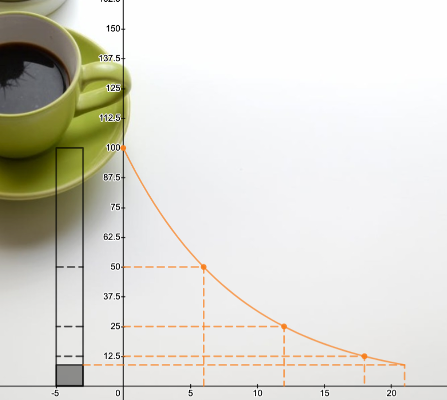
\includegraphics[width=250bp]{cafeina.png}
\caption{Gráfico mostrando como a quantidade de cafeína no organismo de um indivíduo que ingeriu uma xícara de café de $250 ml$ varia ao longo do tempo (medido em horas).}
\end{figure}

Para um indivíduo que acabou de ingerir uma xícara de café de $250 ml$ - que contém cerca de $100 mg$ de cafeína - exames laboratoriais mostraram que a quantidade de cafeína no seu organismo variou com o passar do tempo (em horas) de acordo com a seguinte função $f(t)=100 \cdot (0{,}5)^{\frac{t}{6}}$, pergunta-se:

\begin{enumerate}

\item{}
Quais serão as quantidades de cafeína no organismo deste indivíduo após meia hora, uma hora e meia e quatro horas desde a ingestão da xícara de café ?

\item{}
Quanto tempo deverá se passar desde a ingestão da xícara de café até que a quantidade de cafeína no organismo deste indivíduo caia para a metade da quantidade inicial ?

\item{}
Que mudanças deveríamos fazer na expressão caso a meia-vida da cafeína neste indivíduo fosse de $8$ horas e ele tivesse ingerido 150 mg de cafeína?

\end{enumerate}

\ifdefined\prof
\begin{solucao}

\begin{enumerate}
\item
As quantidades de cafeína no organismo do indivíduo meia hora (0,5), uma hora e meia (1,5) e quatro horas (4) após a ingestão da xícara de café serão, respectivamente, dadas por:

$f(0,5)=94{,}39$mg, \quad $f(1,5)=84{,}09$mg, \quad $f(4)=63$mg.

\item $50=100\cdot(0,5)^{\frac{t}{6}}\iff\dfrac{1}{2}=\left( \dfrac{1}{2} \right)^{\frac{t}{6}}$ $\iff$ $t=6$ horas.

\item $F(t)=150\cdot(0{,}5)^{\frac{t}{8}}$.
\end{enumerate}

\end{solucao}
\fi

\end{document}